\section{Aufbau}
\label{sec:Aufbau}
Ein Signal, welches zuvor durch einen Bandpassfilter von höher- ($\omega \gg \omega_0$) und niederfrequentem ($\omega \ll \omega_0$) Rauschen befreit wurde, wird mit einem Referenzsignal moduliert. Dieses kann durch einen Phasenschieber an das zu messende Signal angeglichen werden, sodass die Schwingungen in Phase sind ($\Delta \phi = 0$). Zuletzt wird das Mischsignal mit einem Tiefpassfilter über mehrere Perioden aufintegriert, wobei sich die stochastischen Rauschanteile bei ausreichender Zeitkonstante $\tau = RC \gg \sfrac{1}{\omega_0}$ aufheben.

\begin{figure}
  \centering
  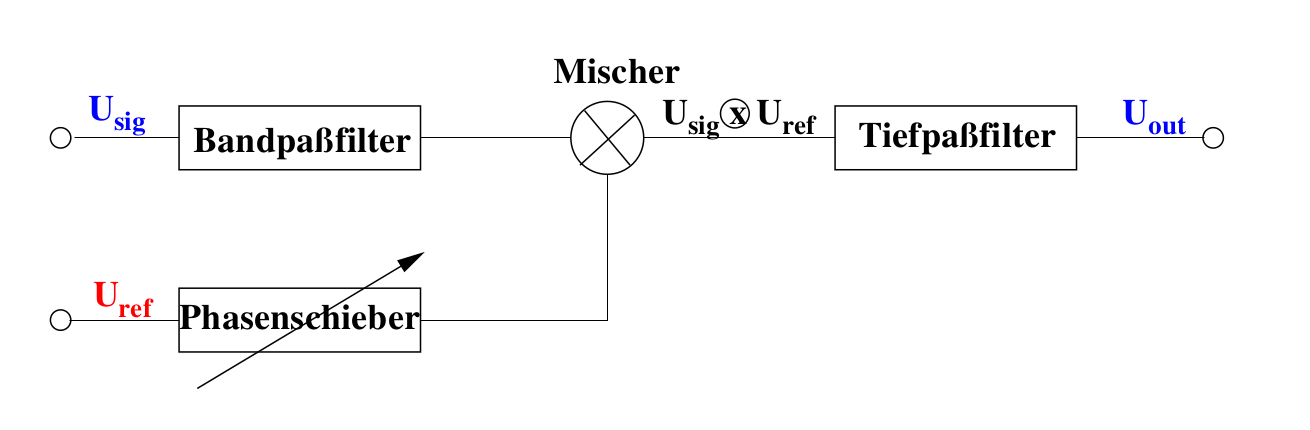
\includegraphics[width=\textwidth]{content/grafiken/Schema.png}
  \caption{Schematische Darstellung eines Lock-In-Verstärkers. Aus \cite{anleitung303}.}
  \label{fig:schema}
\end{figure}


\section{Durchführung}
\label{sec:Durchführung}

Im Experiment wird das in Abb.~\ref{fig:lockin} dargestellte Gerät verwendet, um die Eigenschaften eines Lock-In-Verstärkers zu evaluieren. Es besteht aus Signal- und Rauschgenerator, Vorverstärker, Bandpass, Referenzgenerator, Phasenschieber, Lock-In-Detektor und Tiefpass. Diese können mit Koaxialkabeln untereinander verbunden werden. Die erzeugten Spannungsverläufe werden mithilfe eines digitalen Speicheroszilloskops angezeigt und gespeichert werden.

\subsection{Verrauschtes Signal}
Zuerst wird die Schaltung aus Abb.~\ref{fig:aufbau} aufgebaut und die Funktionsweise des Lock-In-Verstärkers für ein Signal ohne und mit Rauschen evaluiert. Dazu wird der Rauschgenerator zuerst überbrückt, verschiedene Phasenverschiebungen eingestellt und die Ausgangsspannung gemessen. Dieses wird mit nicht überbrücktem Rauschgenerator wiederholt.

\subsection{Photodetektorschaltung}
Danach folgt die Messung einer Photodetektorschaltung mit dem Aufbau aus Abb.~\ref{fig:aufbau2}. Dabei wird die Intensität einer LED, die moduliert angesteuert wird, mit dem Lock-In-Verstärker gemessen.

\begin{figure}
  \centering
  \includegraphics[width=\textwidth]{content/grafiken/Gerät.png}
  \caption{Lock-In-Verstärker.Aus \cite{anleitung303}.}
  \label{fig:lockin}
\end{figure}

\begin{figure}
  \centering
  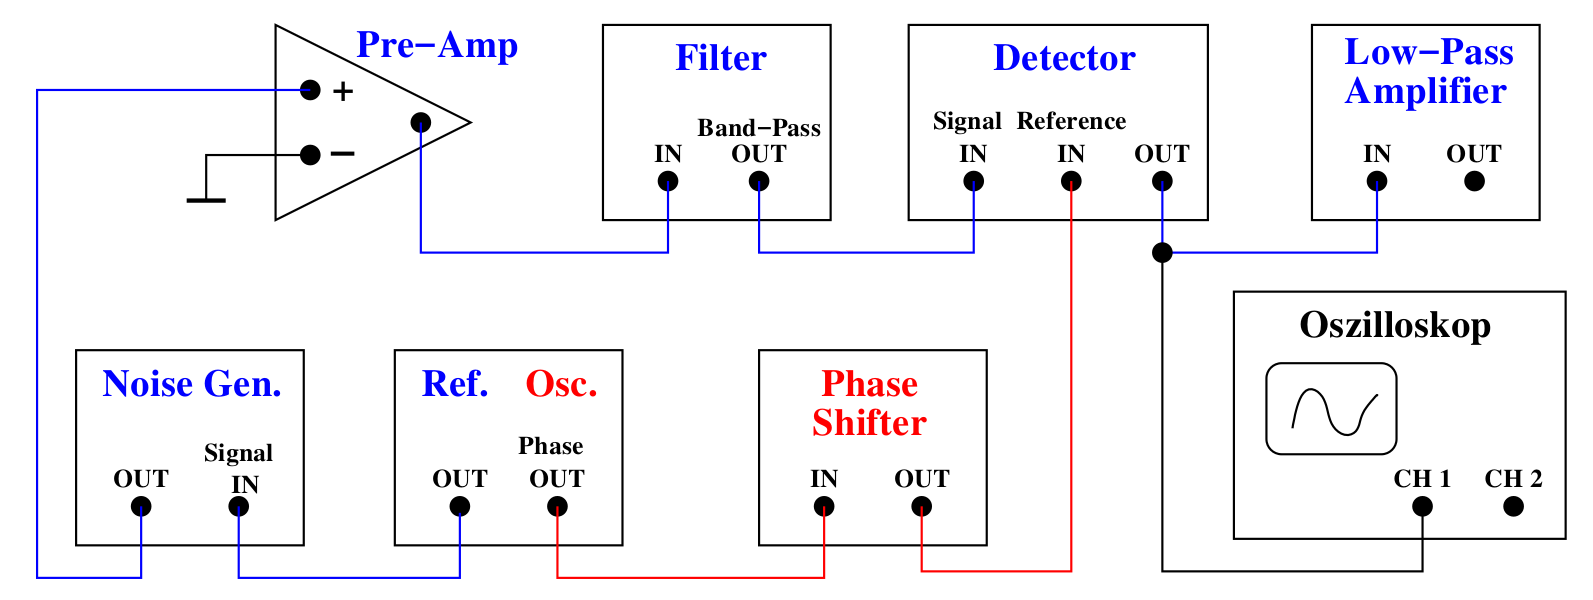
\includegraphics[width=\textwidth]{content/grafiken/Aufbau.png}
  \caption{Schematischer Versuchsaufbau.Aus \cite{anleitung303}.}
  \label{fig:aufbau}
\end{figure}

\begin{figure}
  \centering
  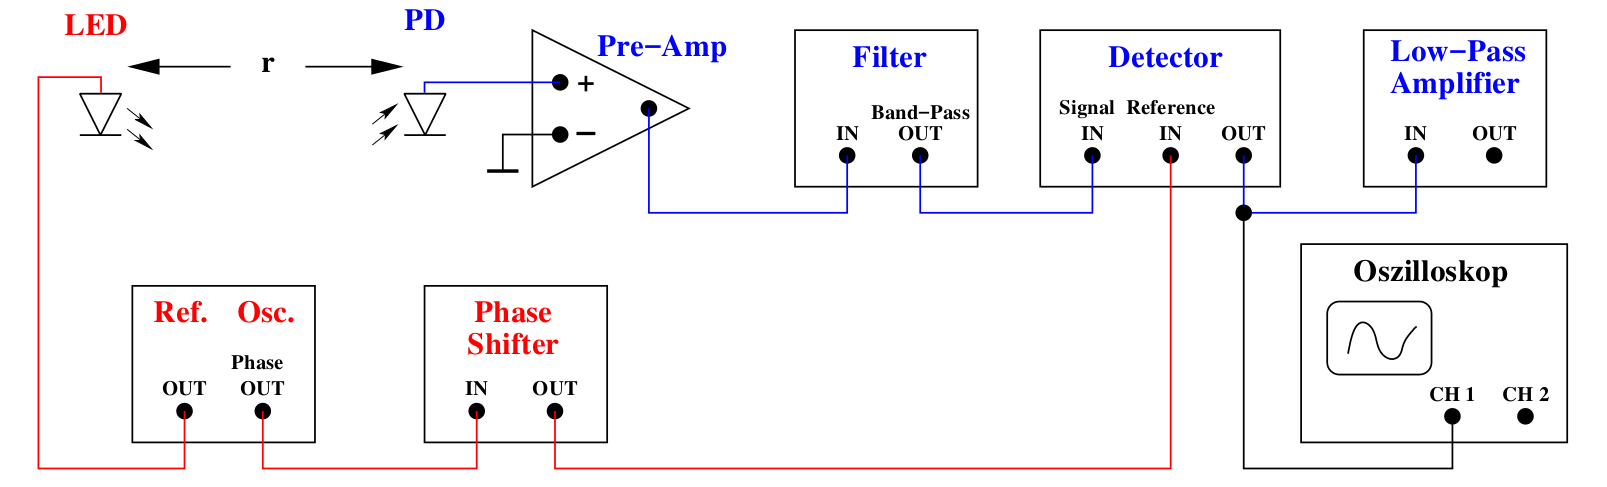
\includegraphics[width=\textwidth]{content/grafiken/Aufbau2.png}
  \caption{Schematischer Versuchsaufbau der Photodetektorschaltung.Aus \cite{anleitung303}.}
  \label{fig:aufbau2}
\end{figure}
